\documentclass[10pt,conference]{IEEEtran}

\usepackage{amsmath}
\usepackage{booktabs}
\usepackage{graphicx}
\usepackage{placeins}
\usepackage{xcolor}
\setlength{\emergencystretch}{1.5em}

% Generated by scripts/41_build_manuscript_assets.py
\newcommand{\FrozenFprTarget}{1\%}
\newcommand{\NoveltyCoverageFloor}{0.80}
\newcommand{\SourceCompetenceTprFloor}{0.10}
\newcommand{\SourceCompetenceFprCeiling}{0.05}
\newcommand{\DatasetCount}{3}
\newcommand{\DirectionCount}{6}
\newcommand{\ModelCount}{4}
\newcommand{\NaturalSettingCount}{24}
\newcommand{\PrimaryIotSettingCount}{8}
\newcommand{\CompetentSourcePairCount}{9}
\newcommand{\NonCompetentSourcePairCount}{3}
\newcommand{\CompetentSettingCount}{18}
\newcommand{\CompetentRankingFailureCount}{15}
\newcommand{\CompetentCollapseCount}{14}
\newcommand{\CompetentInversionCount}{14}
\newcommand{\CompetentRobustInversionCount}{13}
\newcommand{\CompetentSourcePositiveMedianGapCount}{18}
\newcommand{\CompetentInversionMedianCrossoverCount}{12}
\newcommand{\CompetentIotOnlySettingCount}{6}
\newcommand{\CompetentIotOnlyRankingFailureCount}{3}
\newcommand{\CompetentIotOnlyNonCollapsedCount}{3}
\newcommand{\CompetentUnswStressTestSettingCount}{12}
\newcommand{\CompetentUnswStressTestRankingFailureCount}{12}
\newcommand{\FullRankingFailureCount}{20}
\newcommand{\FullCollapseCount}{19}
\newcommand{\FullInversionCount}{19}
\newcommand{\FullRobustInversionCount}{18}
\newcommand{\FullSourcePositiveMedianGapCount}{24}
\newcommand{\FullInversionMedianCrossoverCount}{17}
\newcommand{\ThresholdDriftCount}{2}
\newcommand{\UnswTargetSettingCount}{8}
\newcommand{\UnswTargetRankingFailureCount}{8}
\newcommand{\TonToIotRankingFailureCount}{3}
\newcommand{\CompetentMinTargetAuroc}{0.249}
\newcommand{\CompetentMaxTargetAuroc}{0.636}
\newcommand{\CompetentTargetPaucMedian}{0.498}
\newcommand{\CompetentTargetPaucMin}{0.497}
\newcommand{\CompetentTargetPaucMax}{0.535}
\newcommand{\CompetentSourcePaucMedian}{0.877}
\newcommand{\CompetentNonCollapsedCount}{3}
\newcommand{\CompetentNonCollapsedTargetPaucMin}{0.500}
\newcommand{\CompetentNonCollapsedTargetPaucMax}{0.507}
\newcommand{\CompetentNonCollapsedSourcePaucMedian}{0.909}
\newcommand{\CompetentMedianTargetTpr}{0.165}
\newcommand{\CompetentMedianRealizedFpr}{0.276}
\newcommand{\CompetentSourceFprMin}{0.004}
\newcommand{\CompetentSourceFprMax}{0.010}
\newcommand{\RecalibrationEvalFprMax}{0.022}
\newcommand{\RecalibrationEvalFprExceedanceCount}{9}
\newcommand{\RecalibrationPartitionScoreKsMedian}{0.013}
\newcommand{\RecalibrationPartitionScoreKsMax}{0.292}
\newcommand{\CatastrophicAllNaturalCount}{17}
\newcommand{\CatastrophicPrimaryIotCount}{6}
\newcommand{\WithinHoldoutMin}{0.000}
\newcommand{\WithinHoldoutMax}{0.996}
\newcommand{\AllNaturalMedianTargetTpr}{0.090}
\newcommand{\AllNaturalMedianRealizedFpr}{0.184}
\newcommand{\AllNaturalMinTargetTpr}{0.000}
\newcommand{\AllNaturalMaxTargetTpr}{0.948}
\newcommand{\AllNaturalMinRealizedFpr}{0.000}
\newcommand{\AllNaturalMaxRealizedFpr}{0.919}
\newcommand{\PrimaryOracleSpearman}{0.436}
\newcommand{\DirectionOracleSpearman}{0.926}
\newcommand{\DirectionBenignKsFprSeveritySpearman}{-0.359}
\newcommand{\IotToTonOracleAlpha}{0.426}
\newcommand{\IotToTonMeanRelativeTprDrop}{0.708}
\newcommand{\IotToTonMeanTargetTpr}{0.166}
\newcommand{\IotToTonMeanRealizedFpr}{0.093}
\newcommand{\TonToIotOracleAlpha}{0.000}
\newcommand{\TonToIotMeanRelativeTprDrop}{0.276}
\newcommand{\TonToIotMeanTargetTpr}{0.693}
\newcommand{\TonToIotMeanRealizedFpr}{0.645}
\newcommand{\IotPairMeanKs}{0.26}
\newcommand{\UnswDirectionMeanKsMin}{0.48}
\newcommand{\UnswDirectionMeanKsMax}{0.54}
\newcommand{\AlphaHatAllNaturalCatastrophicAuroc}{0.403}
\newcommand{\AlphaHatAllNaturalCatastrophicAuprc}{0.696}
\newcommand{\AlphaHatAllNaturalSeveritySpearman}{-0.184}
\newcommand{\ProxyAAllNaturalCatastrophicAuroc}{0.349}
\newcommand{\ProxyAAllNaturalCatastrophicAuprc}{0.665}
\newcommand{\ProxyAAllNaturalSeveritySpearman}{-0.228}
\newcommand{\WassersteinAllNaturalCatastrophicAuroc}{0.382}
\newcommand{\SourceRiskAllNaturalCatastrophicAuroc}{0.492}
\newcommand{\AlphaHatPrimaryCatastrophicAuroc}{0.500}
\newcommand{\AlphaHatPrimarySeveritySpearman}{-0.078}
\newcommand{\SourceRiskPrimaryCatastrophicAuroc}{0.333}
\newcommand{\AllNaturalMedianRetunedTargetTpr}{0.002}
\newcommand{\AllNaturalMedianRetunedTprGain}{-0.078}
\newcommand{\IotToTonMedianRetunedTprGain}{-0.048}
\newcommand{\TonToIotMedianRetunedTprGain}{-0.907}
\newcommand{\BudgetHalfPctMedianTargetTpr}{0.047}
\newcommand{\BudgetOnePctMedianTargetTpr}{0.090}
\newcommand{\BudgetFivePctMedianTargetTpr}{0.292}
\newcommand{\BudgetHalfPctMedianRealizedFpr}{0.148}
\newcommand{\BudgetOnePctMedianRealizedFpr}{0.184}
\newcommand{\BudgetFivePctMedianRealizedFpr}{0.318}
\newcommand{\BudgetHalfPctCompetentMedianSourceTpr}{0.778}
\newcommand{\BudgetHalfPctCompetentMedianTargetTpr}{0.080}
\newcommand{\BudgetHalfPctCompetentMedianTargetRealizedFpr}{0.199}
\newcommand{\BudgetHalfPctCompetentMedianBudgetMultiple}{39.831}
\newcommand{\BudgetHalfPctCompetentCatastrophicCount}{12}
\newcommand{\BudgetOnePctCompetentMedianSourceTpr}{0.806}
\newcommand{\BudgetOnePctCompetentMedianTargetTpr}{0.165}
\newcommand{\BudgetOnePctCompetentMedianTargetRealizedFpr}{0.276}
\newcommand{\BudgetOnePctCompetentMedianBudgetMultiple}{27.585}
\newcommand{\BudgetOnePctCompetentCatastrophicCount}{12}
\newcommand{\BudgetFivePctCompetentMedianSourceTpr}{0.891}
\newcommand{\BudgetFivePctCompetentMedianTargetTpr}{0.346}
\newcommand{\BudgetFivePctCompetentMedianTargetRealizedFpr}{0.318}
\newcommand{\BudgetFivePctCompetentMedianBudgetMultiple}{6.351}
\newcommand{\BudgetFivePctCompetentCatastrophicCount}{8}
\newcommand{\BudgetHalfPctCompetentDominantFprxDirection}{TON$\to$I23}
\newcommand{\BudgetOnePctCompetentDominantFprxDirection}{TON$\to$I23}
\newcommand{\BudgetFivePctCompetentDominantFprxDirections}{TON$\to$UNSW and TON$\to$I23}
\newcommand{\BudgetFivePctCompetentCatastrophicShare}{44\%}
\newcommand{\CoralCompetentMedianTargetAuroc}{0.469}
\newcommand{\CoralCompetentRankingFailureCount}{13}
\newcommand{\CoralCompetentMedianTargetPauc}{0.498}
\newcommand{\CoralCompetentMedianBudgetMultiple}{41.699}
\newcommand{\CoralCompetentCatastrophicCount}{14}
\newcommand{\CoralCompetentCatastrophicShare}{78\%}
\newcommand{\CoverageSweepStableFloorMin}{0.50}
\newcommand{\CoverageSweepStableFloorMax}{0.80}
\newcommand{\CoverageSweepEmptyFloor}{0.90}
\newcommand{\CanonicalRunId}{benchmark\_ac1ed34837025ec1}


\title{Decomposing Fixed-Threshold Transfer in Tabular Flow-Level NIDS}

\author{Mustafa Ipekbayrak and G{\"u}ls{\"u}m Zeynep G{\"u}rka\c{s}-Ayd{\i}n}

\begin{document}
\maketitle

\begin{abstract}
Cross-dataset evaluations of network intrusion detection systems (NIDS) routinely show degradation under domain shift, but they seldom distinguish threshold miscalibration from loss of ranking quality. We show that in a three-corpus benchmark of fixed-threshold transfer for tabular flow-level NIDS, degradation is dominated by ranking failure rather than threshold drift: of \CompetentSettingCount{} competent transfer settings, \CompetentRankingFailureCount{} fall below target AUROC 0.60, and \CompetentInversionCount{} of those are below chance on point estimates under the transferred score orientation---a distinct subtype of collapse, not a benign-only recalibration problem. Target standardized pAUC@1\% stays on the chance baseline benchmark-wide (range \CompetentTargetPaucMin{}--\CompetentTargetPaucMax{}, median \CompetentTargetPaucMedian{}) against a source-holdout median of \CompetentSourcePaucMedian{}. The benchmark maps IoT-23, ToN-IoT, and UNSW-NB15 to a shared 16-feature flow schema, trains \ModelCount{} tabular classifiers, freezes thresholds on source validation at \FrozenFprTarget{} FPR, and transfers them unchanged across \NaturalSettingCount{} source-target directions. Benign-only threshold reselection does not rescue detection (mean recalibrated TPR 0.013 across all settings), a 0.5\%/1\%/5\% source-side budget sweep does not reverse the conclusion, and a split-matched CORAL auxiliary comparison raises whole-ROC AUROC but leaves low-FPR ranking unchanged and worsens off-budget behavior. Secondary analyses of attack novelty and benign covariate shift are directional rather than general, and none of the four audited target-free monitors is reliable enough for deployment. The contribution is diagnostic: existing threshold-adaptation and whole-ROC alignment tools are insufficient exactly where low-FPR deployment matters, and the orientation-inversion regime narrows the set of repairs that could plausibly recover deployable detection.
\end{abstract}

\section{Introduction}

The instability of operating points across network domains has been a foundational concern in security machine learning since Axelsson~\cite{axelsson2000baserate} quantified the base-rate fallacy and Sommer and Paxson~\cite{sommer2010outside} argued that closed-world evaluations systematically overstate classifier utility. Cross-dataset NIDS generalization has since received sustained attention through inter-dataset evaluation~\cite{dhooge2020inter}, cross-evaluation frameworks~\cite{xenids2022}, common feature-set studies~\cite{commonfeat2022,layeghy2024benchmarking,iwanowski2025choice}, and threshold adaptation under concept drift~\cite{jordaney2017transcend}. These works document that performance degrades under domain shift. What they do not address is the operational decomposition of that degradation.

When a threshold trained on one network is deployed unchanged on another, the resulting target behavior can fail in three operationally distinct ways under the transferred score rule. \emph{Threshold drift} means the ranking remains usable, but the source-calibrated operating point falls in the wrong region of the target score distribution; this is in principle repairable by recalibrating the threshold on unlabeled target traffic. \emph{Ranking degradation or at-chance collapse} means the transferred ranking no longer provides enough target discrimination for operational repair at the deployment budget, so threshold movement alone cannot recover useful detection. A stricter collapse case is \emph{orientation inversion}: target AUROC falls below chance, indicating that the transferred score direction is reversed relative to the target labels. Inversion is therefore a distinct subtype of collapse within ranking failure, not a benign-only recalibration problem or a label-free repair path.

Prior cross-dataset studies do not make this decomposition, leaving open whether the observed degradation is a fixable calibration problem, a broader ranking failure, or a below-chance inversion under the transferred score orientation. This paper answers the question directly in a three-corpus benchmark. It builds a controlled experiment across IoT-23, ToN-IoT, and UNSW-NB15 using a shared tabular feature schema, \ModelCount{} classifiers, and \CompetentSettingCount{} transfer settings from source-model pairs that pass a predeclared competence rule, then tests benign-only threshold reselection as the simplest realistic repair.

The paper contributes three findings:

\begin{enumerate}
    \item \textbf{Combined low-FPR evidence points to ranking failure, usually via inversion.} Under the paper's coarse AUROC taxonomy, \CompetentRankingFailureCount{} of \CompetentSettingCount{} settings fall below target AUROC 0.60. On point estimates, \CompetentInversionCount{} of those failing settings fall strictly below chance, indicating inverted score orientation under the transferred rule; the remaining failing setting is degraded but not inverted. All \CompetentUnswStressTestRankingFailureCount{} of \CompetentUnswStressTestSettingCount{} UNSW-related stress-test transfers fail, while the \CompetentIotOnlySettingCount{} IoT-only competent transfers split \CompetentIotOnlyRankingFailureCount{} ranking failures and \CompetentIotOnlyNonCollapsedCount{} rows above the 0.60 failure floor. Across all \CompetentSettingCount{} competent settings, target pAUC@1\% stays near the chance baseline (\CompetentTargetPaucMin{}--\CompetentTargetPaucMax{}, median \CompetentTargetPaucMedian{}; source-holdout median \CompetentSourcePaucMedian{}), and neither benign-only recalibration nor diagnostic oracle retuning restores useful sensitivity at \FrozenFprTarget{}. No setting retains ``acceptable'' ranking quality (AUROC $\geq$ 0.70).
    \item \textbf{Benign-only threshold reselection does not rescue the benchmark.} Re-selecting the threshold on target benign traffic at \FrozenFprTarget{} FPR keeps mean recalibrated TPR at 0.013 across all \NaturalSettingCount{} settings, and the held-out benign Eval FPR exceeds the nominal budget in \RecalibrationEvalFprExceedanceCount{} settings (maximum \RecalibrationEvalFprMax{}).
    \item \textbf{Secondary diagnostics remain limited.} A two-direction contrast suggests attack-label novelty and benign covariate shift align with different failure dimensions, but the evidence is narrow, and none of the four audited target-free monitors reaches deployable strength.
\end{enumerate}

\section{Related Work}

\subsection{Operational Evaluation and Cross-Dataset NIDS}

Operational IDS evaluation requires reporting at the false-positive budget that governs deployment, not ranking summaries alone~\cite{axelsson2000baserate,fawcett2006roc,davis2006pr}. In network security, that requirement is especially important because traffic mix, label quality, and capture conditions vary across corpora~\cite{ring2019survey}, and ML-for-security methodology studies have repeatedly flagged closed-world and single-dataset evaluation as overstating utility~\cite{sommer2010outside,arp2022dodo}.

Cross-dataset NIDS evaluation has progressed from single-corpus benchmarks to systematic inter-dataset testing~\cite{dhooge2020inter,xenids2022}. Common feature-set proposals aim to make cross-dataset results comparable~\cite{commonfeat2022}, but recent work continues to report substantial generalization gaps even under shared schemas~\cite{layeghy2024benchmarking,iwanowski2025choice}. These studies establish that aggregate performance drops under transfer; they do not separate threshold miscalibration from ranking failure, nor do they audit behavior at a fixed low-FPR deployment budget under the transferred score orientation.

\subsection{Domain Adaptation and Threshold Repair}

Domain-adaptation methods for NIDS span feature-level alignment~\cite{xdomain2023}, correlation alignment~\cite{sun2016return}, domain-invariant representation learning~\cite{dinids2021}, and adversarial domain-invariant training~\cite{ganin2015dann}. These methods typically optimize whole-ROC accuracy rather than low-FPR operating points and assume that the target score ranking still carries positive information about the target label. Threshold-adaptation under concept drift has been studied explicitly in the malware setting~\cite{jordaney2017transcend,barbero2022transcending}, with selective prediction proposed as a hedge when ranking weakens. Calibration under distribution shift has been addressed through temperature scaling and post-hoc calibration~\cite{guo2017calibration,ovadia2019uncertainty}, all of which presuppose a monotone relationship between the transferred score and the target label that the orientation-inversion regime documented here violates.

\subsection{Shift Detection and Unlabeled-Data Monitors}

Domain classifiers, feature-distribution distances, and calibration diagnostics are standard monitor inputs under domain shift~\cite{ben2010domain,ovadia2019uncertainty,rabanser2019failing,hendrycks2017baseline}. A recent cyberthreat-detection SoK surveys what unlabeled target data can and cannot establish about deployed detector quality~\cite{apruzzese2023realgap}. Section~\ref{sec:monitors} compares four such target-free scores against operational severity in this benchmark and finds none deployably reliable, consistent with that SoK's conclusion that unlabeled data is a weak instrument for deployability claims.

\subsection{Positioning of This Paper}

This paper complements rather than competes with the adaptation and monitoring literature. It does not propose a new method. Instead, it establishes that the operational failure observed under cross-dataset fixed-threshold transfer in this benchmark is predominantly a ranking-quality failure, frequently with inverted score orientation under the transferred rule. That diagnosis narrows the set of repairs that could plausibly recover deployable detection: benign-only threshold reselection and whole-ROC alignment are insufficient in this benchmark, while methods that can re-orient the score direction---target-labeled adaptation, explicit semantic alignment, or supervised calibration on a small target sample---remain the open path.

\section{Experimental Design}

\subsection{Datasets and Tiered Analysis}

The experiment uses three public datasets arranged in two tiers~\cite{garcia2020iot23,booij2022ton,moustafa2015unsw}. \emph{Tier~1} (full experiment) includes all \DirectionCount{} ordered directions across IoT-23, ToN-IoT, and UNSW-NB15, yielding \NaturalSettingCount{} raw settings. \emph{Tier~2} (claim-bearing novelty subset) restricts to the \PrimaryIotSettingCount{} IoT-only settings where the coarse attack ontology achieves mapped coverage above \NoveltyCoverageFloor{} on both domains. Oracle novelty claims are made only on Tier~2. UNSW-NB15 is retained in Tier~1 as a stress-test domain but is not a semantic peer in the novelty analysis.

\subsection{Feature Schema and Protocol}

All datasets are first reduced to one shared flow-level primitive schema (record\_id, group\_id, label, family\_raw, proto, duration\_s, src\_bytes, dst\_bytes, src\_pkts, dst\_pkts) and then mapped deterministically into feature\_schema\_v1, the canonical 16-feature tabular flow-level NIDS representation used throughout the benchmark.

% Generated by src/iot_ids/schema_appendix.py
\begin{table*}[!tbp]
\centering
\scriptsize
\renewcommand{\arraystretch}{1.08}
\setlength{\tabcolsep}{4pt}
\caption{Shared-schema quantitative features used in the canonical benchmark (feature schema v1).}
\label{tab:shared-feature-schema-quantitative}
\begin{tabular}{p{0.17\textwidth}p{0.55\textwidth}p{0.22\textwidth}}
\toprule
Feature & Formula & Derived From \\
\midrule
log\_duration\_s & log1p(max(duration\_s, 0)) & duration\_s \\
log\_src\_bytes & log1p(max(src\_bytes, 0)) & src\_bytes \\
log\_dst\_bytes & log1p(max(dst\_bytes, 0)) & dst\_bytes \\
log\_src\_pkts & log1p(max(src\_pkts, 0)) & src\_pkts \\
log\_dst\_pkts & log1p(max(dst\_pkts, 0)) & dst\_pkts \\
log\_total\_bytes & log1p(src\_bytes + dst\_bytes) & src\_bytes, dst\_bytes \\
log\_total\_pkts & log1p(src\_pkts + dst\_pkts) & src\_pkts, dst\_pkts \\
log\_bytes\_per\_s & log1p((src\_bytes + dst\_bytes) / duration\_s); 0 when duration\_s = 0 & duration\_s, src\_bytes, dst\_bytes \\
log\_pkts\_per\_s & log1p((src\_pkts + dst\_pkts) / duration\_s); 0 when duration\_s = 0 & duration\_s, src\_pkts, dst\_pkts \\
src\_byte\_frac & src\_bytes / (src\_bytes + dst\_bytes); 0.5 when total\_bytes = 0 & src\_bytes, dst\_bytes \\
src\_pkt\_frac & src\_pkts / (src\_pkts + dst\_pkts); 0.5 when total\_pkts = 0 & src\_pkts, dst\_pkts \\
bytes\_per\_pkt & (src\_bytes + dst\_bytes) / (src\_pkts + dst\_pkts); 0 when total\_pkts = 0 & src\_bytes, dst\_bytes, src\_pkts, dst\_pkts \\
\bottomrule
\end{tabular}
\end{table*}


Table~\ref{tab:shared-feature-schema-quantitative} lists the 12 quantitative derived features. The protocol field is one-hot encoded into four canonical indicators: proto\_tcp, proto\_udp, proto\_icmp, and proto\_other. The dataset-to-primitive mapping rules and source-side staged columns discarded before the shared schema remain in the generated artifact package. No dataset-specific feature branch is allowed in the canonical run. Each source dataset is split deterministically into train (60\%), validation (20\%), and holdout (20\%) partitions using the staged group\_id as the split and grouped-bootstrap unit. In the current staging code, this is connection-level for IoT-23 and ToN-IoT and effectively row-level for UNSW-NB15: IoT-23 uses capture\_id concatenated with the 5-tuple and protocol, ToN-IoT uses the 5-tuple and protocol, and UNSW-NB15 uses record\_id. Operating-point confidence intervals therefore resample those same group\_id units at 95\% with 2000 resamples. The monitor-audit intervals in Table~\ref{tab:monitor} instead use bootstrap over transfer settings with 5000 resamples.

The experiment trains \ModelCount{} tabular baselines spanning linear, ensemble, and neural settings. For each source-model pair, the threshold is fixed once on source-validation negatives at \FrozenFprTarget{} FPR and transferred unchanged. All threshold selection uses a tie-safe rule consistent with predictions of the form score $\geq$ threshold: choose the smallest cutoff whose realized FPR under that rule does not exceed the budget; if a tied block of negative scores straddles the budget, move the cutoff strictly above that tied score so the whole tie block remains negative. For low-FPR ranking checks aligned with the deployment budget, the paper also reports pAUC@1\%, defined here as the standardized partial AUROC over FPR~$\leq$~\FrozenFprTarget{} under the transferred score orientation; on this scale, 0.5 is chance-level low-FPR ranking and 1.0 is perfect low-FPR ranking. To test whether the deployment conclusion is tied to the nominal operating point, the same frozen source-threshold transfer protocol is additionally audited at 0.5\%, 1\%, and 5\% source-validation FPR budgets, transferring each source-selected threshold unchanged to source holdout and target. As one auxiliary unlabeled adaptation check, CORAL is fit using source-train features and a deterministic 50/50 target-test adaptation half split by group, then evaluated on the disjoint target-evaluation half under the same frozen \FrozenFprTarget{} source-validation threshold rule.

\subsection{Source-Model Competence Filter}

The competent-setting subset is defined by a source-side rule applied before transfer interpretation. A source-model pair is marked non-competent if its source-holdout TPR@\FrozenFprTarget{} is below \SourceCompetenceTprFloor{}, if its source-holdout realized FPR exceeds \SourceCompetenceFprCeiling{}, or if the frozen threshold is saturated at the top of the score range and still violates the nominal \FrozenFprTarget{} budget. This excludes \NonCompetentSourcePairCount{} source-model pairs and leaves \CompetentSettingCount{} competent transfer settings from \CompetentSourcePairCount{} competent source-model pairs. All full-benchmark (\NaturalSettingCount{}-setting) results are still reported in parallel throughout the paper.

% Generated by scripts/41_build_manuscript_assets.py
\begin{table}[htbp]
\centering
\footnotesize
\setlength{\tabcolsep}{4pt}
\caption{Source-side quality. TPR and FPR are at the frozen \FrozenFprTarget{} threshold. Rows marked with $\dagger$ fail the metric-derived competence rule used for the competent-setting subset.}
\label{tab:source}
\begin{tabular}{llrrr}
\toprule
Dataset & Model & AUROC & TPR [95\% CI] & FPR \\
\midrule
I23 & LR & 0.805 & 0.521 [0.519, 0.522] & 0.010 \\
 & ET$\dagger$ & 0.875 & 0.000 [0.000, 0.000] & 0.000 \\
 & HGB & 0.988 & 0.953 [0.953, 0.954] & 0.010 \\
 & MLP & 0.971 & 0.773 [0.772, 0.774] & 0.008 \\
TON & LR$\dagger$ & 0.977 & 0.080 [0.076, 0.085] & 0.006 \\
 & ET & 0.999 & 0.996 [0.993, 0.998] & 0.004 \\
 & HGB & 1.000 & 0.993 [0.989, 0.995] & 0.006 \\
 & MLP & 0.997 & 0.968 [0.964, 0.971] & 0.007 \\
UNSW & LR & 0.893 & 0.245 [0.241, 0.250] & 0.008 \\
 & ET$\dagger$ & 0.975 & 0.000 [0.000, 0.000] & 0.000 \\
 & HGB & 0.981 & 0.806 [0.802, 0.811] & 0.009 \\
 & MLP & 0.955 & 0.624 [0.619, 0.629] & 0.007 \\
\bottomrule
\end{tabular}
\end{table}


\subsection{Unlabeled Recalibration Baseline}

For each setting, the threshold is re-selected at \FrozenFprTarget{} FPR using only target benign traffic (no attack labels). The target benign pool is partitioned deterministically into a calibration split for threshold selection and a disjoint evaluation split for the realized benign FPR estimate. In practice, this corresponds to a short known-clean deployment window plus a held-out benign audit slice. The same tie-safe threshold rule used for source-side freezing is applied here. Benign-only threshold reselection can improve the operating point only when low-FPR discrimination remains usable; if ranking has collapsed, threshold reselection cannot restore useful sensitivity at the \FrozenFprTarget{} budget. This is the simplest realistic repair.

\subsection{Oracle Novelty}
\label{sec:oracle-novelty-def}

Oracle novelty $\alpha$ is defined with target labels as the fraction of target attacks whose ontology group is unseen in the source training set. This analysis uses target labels and is therefore a diagnostic tool, not a deployable one. The analysis is claim-bearing only on Tier~2 (the \PrimaryIotSettingCount{} IoT-only settings where both source and target mapped attack coverage exceeds \NoveltyCoverageFloor{}).

\subsection{Target-Free Monitors}
\label{sec:monitors}

We audit four unlabeled monitors against the operational failure targets:

\textbf{Target-free novelty proxy ($\hat{\alpha}$).} A $k$-NN model ($k{=}10$) fitted on source-train attacks, with cutoff at the $0.95$ quantile of leave-one-out source distances. It scores the fraction of target predicted-positives whose $k$-NN distance exceeds the cutoff. This is a pre-specified heuristic baseline with frozen hyperparameters, not a proposed method. By design, $\hat{\alpha}$ measures attack-side novelty only; benign covariate shift is outside its line of sight.

\textbf{Proxy-A distance ($d_A$).} A logistic domain classifier; $d_A = \max(0, 2(1 - 2\,\mathrm{err}))$.

\textbf{Average Wasserstein distance.} Average feature-wise transport distance (1D Wasserstein) between source-train and target.

\textbf{Source-validation risk.} Negated source-validation TPR---a trivial baseline.

\subsection{Evaluation Targets}

The monitors are evaluated against two operational targets.

\textbf{Operational severity} is the maximum of relative TPR drop and FPR severity:
\[
\mathrm{severity} = \max(\mathrm{relative\ TPR\ drop},\ \mathrm{FPR\ severity}).
\]
Relative TPR drop is
\[
\max(0,\, 1 - \mathrm{TPR}_{\mathrm{target}} / \mathrm{TPR}_{\mathrm{source}}),
\]
and FPR severity is
\[
\min(1,\, \max(0,\, \mathrm{FPR}_{\mathrm{target}} / 0.01 - 1) / 9).
\]
This stylized composite is a reporting summary, not a validated incident-cost model.

\textbf{Catastrophic operational failure} $= \mathbf{1}[\text{severity} \geq 1]$.

\section{Results}

\subsection{Source-Side Sanity}

Table~\ref{tab:source} shows that the \CompetentSourcePairCount{} competent source-model pairs all achieve AUROC above 0.80 and source-holdout FPR near the intended \FrozenFprTarget{} budget (range \CompetentSourceFprMin{}--\CompetentSourceFprMax{}). The threshold calibration therefore holds within-domain on the rows that enter the competent-setting analysis. Rows marked with $\dagger$ fail the source-side competence rule and are shown for completeness.

\FloatBarrier

\subsection{Full Cross-Domain Transfer}

\begin{figure}[t]
\centering
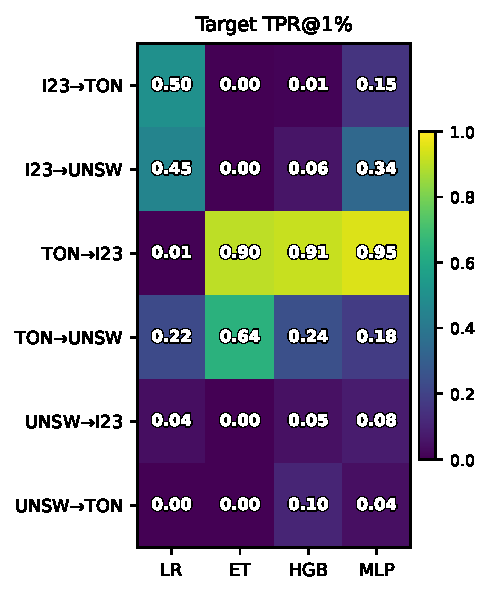
\includegraphics[width=\columnwidth]{figures/transfer_tpr.pdf}
\caption{Tier~1 benchmark: target TPR at the frozen \FrozenFprTarget{} source-validation threshold, across \DirectionCount{} directions $\times$ \ModelCount{} classifiers. Most cells are near zero. The apparent exception is the TON$\to$I23 row (TPR 0.90--0.95 for ET/HGB/MLP), but Fig.~\ref{fig:transfer-fpr} shows the same row operates far off the \FrozenFprTarget{} FPR budget on target, so high TPR there is not deployable detection.}
\label{fig:transfer-tpr}
\end{figure}

\begin{figure}[t]
\centering
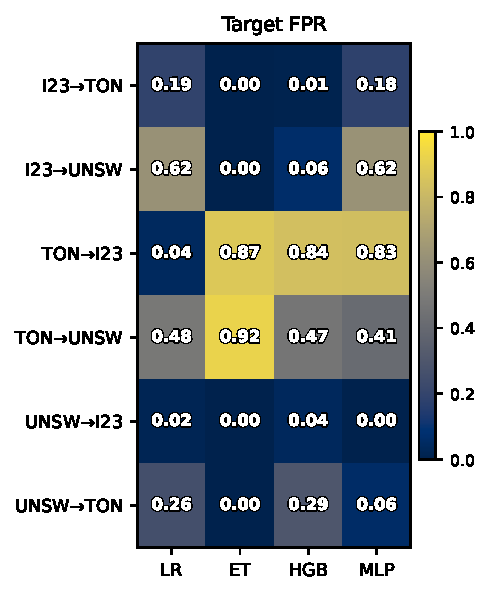
\includegraphics[width=\columnwidth]{figures/transfer_fpr.pdf}
\caption{Tier~1 benchmark: realized target FPR under the transferred threshold. Cells near or above the \FrozenFprTarget{} budget (notably TON$\to$I23 at 0.83--0.87 and the LR column of I23$\to$UNSW, TON$\to$UNSW) indicate the source-calibrated operating point does not hold on target; cells near zero indicate the opposite failure mode---a saturated threshold that produces almost no alerts.}
\label{fig:transfer-fpr}
\end{figure}

Across all \NaturalSettingCount{} raw settings, median target TPR is \AllNaturalMedianTargetTpr{} and median realized FPR is \AllNaturalMedianRealizedFpr{} (Figures~\ref{fig:transfer-tpr} and~\ref{fig:transfer-fpr}). On the \CompetentSettingCount{} competent settings, median target TPR rises slightly to \CompetentMedianTargetTpr{} and median realized FPR to \CompetentMedianRealizedFpr{}.

% Generated by scripts/41_build_manuscript_assets.py
\begin{table}[htbp]
\centering
\scriptsize
\setlength{\tabcolsep}{4pt}
\caption{Direction-level transfer summary across the 4 canonical models. The full per-setting matrix remains in the artifact package; this table provides a compact directional view. The two IoT-only directions carry the novelty interpretation, while the UNSW-NB15 directions remain stress tests.}
\label{tab:acsac-cross-summary}
\begin{tabular}{lrrrr}
\toprule
Direction & Med TPR & Med FPR & Min TPR & Max FPR \\
\midrule
I23$\to$TON & 0.081 & 0.092 & 0.000 & 0.189 \\
I23$\to$UNSW & 0.197 & 0.340 & 0.000 & 0.618 \\
TON$\to$I23 & 0.907 & 0.833 & 0.007 & 0.875 \\
TON$\to$UNSW & 0.233 & 0.476 & 0.177 & 0.919 \\
UNSW$\to$I23 & 0.042 & 0.011 & 0.000 & 0.038 \\
UNSW$\to$TON & 0.022 & 0.157 & 0.000 & 0.295 \\
\bottomrule
\end{tabular}
\end{table}


\subsection{Ranking Failure Taxonomy}
\label{sec:ranking-diagnosis}

We classify each setting by its target AUROC using the Hosmer--Lemeshow discrimination guideline~\cite{hosmer2013applied}: AUROC below 0.60 indicates ranking failure at the paper's coarse discrimination floor. Within that umbrella, AUROC at or below 0.50 is ranking collapse. Exact-chance rows are collapse without usable directional signal, while AUROC below 0.50 is the inverted target score orientation subset of that collapse category under the transferred score rule. Rows with 0.50~$<$~AUROC~$<$~0.60 are degraded rather than collapsed. No setting in this benchmark lies exactly at the AUROC~=~0.50 boundary. This cutoff reflects 60\% pairwise concordance---operationally insufficient for alert-budget deployment.

% Generated by scripts/41_build_manuscript_assets.py
\begin{table}[htbp]
\centering
\scriptsize
\setlength{\tabcolsep}{3pt}
\caption{Source vs.\ target AUROC for the 18 competent settings. Ranking failure ($\dagger$: target AUROC~$<$~0.60); inversion ($\ddagger$: target AUROC~$<$~0.50 under the transferred score orientation). Target AUROC intervals are grouped-bootstrap 95\% percentile CIs over the benchmark grouping units, reported as descriptive intervals rather than multiplicity-adjusted inference; markers remain keyed to the point estimates. The final column reports source-holdout / target standardized pAUC@1\%; on this scale, 0.5 denotes chance-level low-FPR ranking. No setting achieves acceptable ranking (AUROC $\geq$ 0.70).}
\label{tab:collapse}
\begin{tabular}{llp{1.40in}r}
\toprule
Direction & Model & Tgt AUROC [95\% CI] & Src/Tgt pAUC@1\% \\
\midrule
I23$\to$TON & LR & 0.636 [0.582, 0.700] & 0.582 / 0.500 \\
 & HGB & 0.617 [0.507, 0.736] & 0.942 / 0.507 \\
 & MLP & 0.559 [0.487, 0.655]$\dagger$ & 0.796 / 0.498 \\
I23$\to$UNSW & LR & 0.360 [0.354, 0.366]$\dagger$$\ddagger$ & 0.582 / 0.503 \\
 & HGB & 0.407 [0.402, 0.412]$\dagger$$\ddagger$ & 0.942 / 0.498 \\
 & MLP & 0.329 [0.325, 0.335]$\dagger$$\ddagger$ & 0.796 / 0.501 \\
TON$\to$I23 & ET & 0.453 [0.450, 0.457]$\dagger$$\ddagger$ & 0.978 / 0.500 \\
 & HGB & 0.427 [0.423, 0.431]$\dagger$$\ddagger$ & 0.982 / 0.498 \\
 & MLP & 0.624 [0.620, 0.628] & 0.909 / 0.500 \\
TON$\to$UNSW & ET & 0.249 [0.244, 0.253]$\dagger$$\ddagger$ & 0.978 / 0.498 \\
 & HGB & 0.360 [0.355, 0.365]$\dagger$$\ddagger$ & 0.982 / 0.497 \\
 & MLP & 0.258 [0.253, 0.262]$\dagger$$\ddagger$ & 0.909 / 0.497 \\
UNSW$\to$I23 & LR & 0.418 [0.414, 0.422]$\dagger$$\ddagger$ & 0.613 / 0.517 \\
 & HGB & 0.375 [0.371, 0.378]$\dagger$$\ddagger$ & 0.877 / 0.498 \\
 & MLP & 0.425 [0.421, 0.429]$\dagger$$\ddagger$ & 0.791 / 0.535 \\
UNSW$\to$TON & LR & 0.386 [0.271, 0.486]$\dagger$$\ddagger$ & 0.613 / 0.498 \\
 & HGB & 0.285 [0.242, 0.342]$\dagger$$\ddagger$ & 0.877 / 0.498 \\
 & MLP & 0.414 [0.304, 0.511]$\dagger$$\ddagger$ & 0.791 / 0.498 \\
\bottomrule
\end{tabular}
\end{table}


\textbf{Ranking failure count.} Table~\ref{tab:collapse} reports grouped-bootstrap 95\% AUROC CIs with source-holdout and target pAUC@1\% for every competent setting. \CompetentRankingFailureCount{} of \CompetentSettingCount{} competent settings fall into ranking failure; source models with AUROC 0.80--1.00 drop to target AUROC \CompetentMinTargetAuroc{}--\CompetentMaxTargetAuroc{}. Only \CompetentNonCollapsedCount{} settings lie above the 0.60 failure floor (I23$\to$TON / LR, I23$\to$TON / HGB, TON$\to$I23 / MLP), and even those remain below the acceptable-ranking threshold on point estimates.

\textbf{Inversion, not just degradation.} Of the \CompetentRankingFailureCount{} failing settings, \CompetentCollapseCount{} are point-estimate collapse rows; since no setting sits exactly at AUROC~=~0.50, all \CompetentCollapseCount{} are below-chance inversions under the transferred score orientation, and \CompetentRobustInversionCount{} retain 95\% AUROC upper bounds below 0.50. The remaining failing setting is degraded but not inverted. A score-space view is consistent: all \CompetentSourcePositiveMedianGapCount{} competent source-holdout rows keep attack median scores above benign medians, while \CompetentInversionMedianCrossoverCount{} of the \CompetentInversionCount{} inversion rows show target benign medians meeting or exceeding target attack medians. Inversion is therefore a score-order reversal under transfer, not a candidate for a deployable sign-flip fix in the source-only setting: correcting orientation without target labels or prior semantic knowledge is outside the scope of fixed-threshold transfer.

\textbf{Where the failures concentrate.} The \CompetentUnswStressTestSettingCount{} UNSW-related stress-test transfers all fail. The \CompetentIotOnlySettingCount{} IoT-only competent settings split \CompetentIotOnlyRankingFailureCount{} failures and \CompetentIotOnlyNonCollapsedCount{} survivors above the floor, indicating that IoT-to-IoT transfer is not uniformly catastrophic but remains non-deployable at the low-FPR budget.

\textbf{Low-FPR ranking is weak benchmark-wide.} Across all \CompetentSettingCount{} competent settings, target pAUC@1\% ranges from \CompetentTargetPaucMin{} to \CompetentTargetPaucMax{} (median \CompetentTargetPaucMedian{}) against a source-holdout median of \CompetentSourcePaucMedian{}---effectively on the chance baseline. Even the \CompetentNonCollapsedCount{} survivors above the 0.60 AUROC floor show target pAUC@1\% only \CompetentNonCollapsedTargetPaucMin{}--\CompetentNonCollapsedTargetPaucMax{} against source-holdout median \CompetentNonCollapsedSourcePaucMedian{}. The \CompetentRankingFailureCount{}/\CompetentSettingCount{} AUROC count is therefore a point-estimate summary; the deployment-facing conclusion rests on benchmark-wide near-chance low-FPR ranking, which neither benign-only recalibration nor oracle retuning repairs at the \FrozenFprTarget{} budget.

% Generated by scripts/41_build_manuscript_assets.py
\begin{table}[htbp]
\centering
\scriptsize
\setlength{\tabcolsep}{3pt}
\caption{Source-selected operating-budget robustness on the 18 competent settings. Each row freezes the threshold at the listed source-validation FPR budget and transfers it unchanged to source holdout and target. FPR$\times$ denotes the median realized target FPR divided by the selected source-side budget. Cat./18 counts catastrophic settings under the existing operational-severity rule.}
\label{tab:acsac-budget-robustness}
\begin{tabular}{lrrrr}
\toprule
Budget & Src med. TPR & Tgt med. TPR & Med. FPR$\times$ & Cat./18 \\
\midrule
0.5\% & 0.778 & 0.080 & 39.831 & 12 \\
1\% & 0.806 & 0.165 & 27.585 & 12 \\
5\% & 0.891 & 0.346 & 6.351 & 8 \\
\bottomrule
\end{tabular}
\end{table}


Table~\ref{tab:acsac-budget-robustness} extends that audit across the 0.5\%/1\%/5\% source-side budget sweep. Looser source budgets raise competent-set median target TPR from \BudgetHalfPctCompetentMedianTargetTpr{} to \BudgetFivePctCompetentMedianTargetTpr{}, but median realized target FPR still remains \BudgetHalfPctCompetentMedianBudgetMultiple{}x to \BudgetFivePctCompetentMedianBudgetMultiple{}x the selected budget and catastrophic failures persist (\BudgetHalfPctCompetentCatastrophicCount{} to \BudgetFivePctCompetentCatastrophicCount{} of \CompetentSettingCount{} settings). The largest FPR$\times$ medians are driven by \BudgetHalfPctCompetentDominantFprxDirection{} at 0.5\%, \BudgetOnePctCompetentDominantFprxDirection{} at 1\%, and \BudgetFivePctCompetentDominantFprxDirections{} at 5\%. Even at 5\%, \BudgetFivePctCompetentCatastrophicCount{} settings remain catastrophic, still \BudgetFivePctCompetentCatastrophicShare{} of the competent set. The deployment-facing conclusion therefore does not reverse across this source-side budget sweep.

% Generated by scripts/41_build_manuscript_assets.py
\begin{table}[htbp]
\centering
\scriptsize
\setlength{\tabcolsep}{3pt}
\caption{Auxiliary unlabeled CORAL comparison on the same 18-setting competent view used by the source-only benchmark. The target-test partition is split deterministically by group into unlabeled adaptation and held-out evaluation halves; both rows are evaluated on the same held-out target half, while CORAL alone fits on the unlabeled adaptation half. CORAL raises whole-ROC AUROC modestly, but it leaves low-FPR pAUC unchanged and worsens FPR$\times$/Cat., so this auxiliary adaptation check supports rather than overturns the deployment diagnosis.}
\label{tab:acsac-coral-auxiliary}
\begin{tabular}{lrrrr}
\toprule
Method & Med. tgt AUROC & Med. tgt pAUC@1\% & Med. FPR$\times$ & Cat./18 \\
\midrule
Source-only & 0.388 & 0.499 & 30.516 & 13 \\
CORAL & 0.469 & 0.498 & 41.699 & 14 \\
\bottomrule
\end{tabular}
\end{table}


Table~\ref{tab:acsac-coral-auxiliary} is a split-matched auxiliary comparison on the same \CompetentSettingCount{} competent settings and held-out target-evaluation halves. In that matched view, CORAL raises median target AUROC but leaves target pAUC@1\% at \CoralCompetentMedianTargetPauc{} while worsening median FPR$\times$ to \CoralCompetentMedianBudgetMultiple{} and increasing catastrophic settings to \CoralCompetentCatastrophicCount{}. This auxiliary adaptation check therefore supports the paper's diagnosis: improving whole-ROC ranking does not recover low-FPR deployability here.

\FloatBarrier

\subsection{Benign-Only Recalibration Does Not Rescue Transfer}
\label{sec:recalibration-results}

% Generated by scripts/46_unlabeled_recalibration.py
\begin{table*}[t]
\centering
\scriptsize
\setlength{\tabcolsep}{5pt}
\caption{Per-setting benign-only recalibration at \FrozenFprTarget{} FPR using only a target-benign calibration split (no attack labels). Recal TPR is measured on the full target attack set, while Eval FPR is measured on a disjoint held-out target-benign evaluation split and printed to four decimals so exceedances just above the \FrozenFprTarget{} budget remain visible. Rows are grouped by transfer direction. The final row reports the mean across all \NaturalSettingCount{} settings.}
\label{tab:acsac-recalibration}
\begin{tabular}{llrrrr}
\toprule
Direction & Model & Target AUROC & Frozen TPR & Recal TPR & Eval FPR \\
\midrule
I23$\to$TON & LR & 0.636 & 0.500 & 0.008 & 0.0178 \\
I23$\to$TON & ET & 0.633 & 0.000 & 0.071 & 0.0051 \\
I23$\to$TON & HGB & 0.617 & 0.010 & 0.066 & 0.0102 \\
I23$\to$TON & MLP & 0.559 & 0.152 & 0.000 & 0.0000 \\
\midrule
I23$\to$UNSW & LR & 0.360 & 0.451 & 0.012 & 0.0104 \\
I23$\to$UNSW & ET & 0.347 & 0.000 & 0.004 & 0.0091 \\
I23$\to$UNSW & HGB & 0.407 & 0.057 & 0.002 & 0.0086 \\
I23$\to$UNSW & MLP & 0.329 & 0.338 & 0.007 & 0.0083 \\
\midrule
TON$\to$I23 & LR & 0.392 & 0.007 & 0.000 & 0.0115 \\
TON$\to$I23 & ET & 0.453 & 0.900 & 0.000 & 0.0000 \\
TON$\to$I23 & HGB & 0.427 & 0.915 & 0.001 & 0.0068 \\
TON$\to$I23 & MLP & 0.624 & 0.948 & 0.013 & 0.0082 \\
\midrule
TON$\to$UNSW & LR & 0.274 & 0.224 & 0.002 & 0.0104 \\
TON$\to$UNSW & ET & 0.249 & 0.639 & 0.001 & 0.0053 \\
TON$\to$UNSW & HGB & 0.360 & 0.243 & 0.000 & 0.0039 \\
TON$\to$UNSW & MLP & 0.258 & 0.177 & 0.000 & 0.0065 \\
\midrule
UNSW$\to$I23 & LR & 0.418 & 0.039 & 0.039 & 0.0095 \\
UNSW$\to$I23 & ET & 0.444 & 0.000 & 0.000 & 0.0078 \\
UNSW$\to$I23 & HGB & 0.375 & 0.045 & 0.003 & 0.0116 \\
UNSW$\to$I23 & MLP & 0.425 & 0.075 & 0.077 & 0.0090 \\
\midrule
UNSW$\to$TON & LR & 0.386 & 0.002 & 0.001 & 0.0171 \\
UNSW$\to$TON & ET & 0.192 & 0.000 & 0.000 & 0.0000 \\
UNSW$\to$TON & HGB & 0.285 & 0.104 & 0.002 & 0.0217 \\
UNSW$\to$TON & MLP & 0.414 & 0.042 & 0.002 & 0.0222 \\
\midrule
\emph{Mean (24)} & -- & 0.411 & 0.245 & 0.013 & 0.0092 \\
\bottomrule
\end{tabular}
\end{table*}


Table~\ref{tab:acsac-recalibration} lists all \NaturalSettingCount{} settings under the benign-only reselection baseline, with the threshold chosen on a deterministic target-benign calibration split and Eval FPR measured on a disjoint held-out benign evaluation split. Benign-only reselection does not rescue the benchmark: no row exceeds recalibrated TPR 0.10, and even the three survivors above the 0.60 failure floor (I23$\to$TON / LR, I23$\to$TON / HGB, TON$\to$I23 / MLP) remain weak after recalibration.

The calibration split respects the budget by construction under the tie-safe rule; the held-out Eval FPR is an audit estimate and exceeds the nominal budget in \RecalibrationEvalFprExceedanceCount{} settings (maximum \RecalibrationEvalFprMax{}). A score-space audit of the calibration-versus-evaluation benign partitions yields median KS \RecalibrationPartitionScoreKsMedian{} and maximum KS \RecalibrationPartitionScoreKsMax{}, so these exceedances are reported descriptively rather than attributed to a single cause. The conclusion does not depend on that audit: recalibrated TPR is too low to change it either way.

This pattern is consistent with representational failure dominating in these settings. When target ranking collapses to chance or below, no threshold can restore useful sensitivity at the \FrozenFprTarget{} budget under the transferred score orientation. When target AUROC survives only in the 0.617--0.636 range, the rows remain above the 0.60 failure floor but their low-FPR discrimination is still too weak to support useful detection at that budget.

% Generated by scripts/41_build_manuscript_assets.py
\begin{table}[htbp]
\centering
\scriptsize
\setlength{\tabcolsep}{4pt}
\caption{Diagnostic oracle retuning at the same \FrozenFprTarget{} false-positive budget. Thresholds are re-selected with target labels for diagnosis only; this table is not part of the frozen-threshold benchmark protocol. The change column reports the median of per-setting retuned-minus-fixed TPR changes within each direction, not the difference between direction medians. When the transferred frozen threshold already runs far above the target-domain \FrozenFprTarget{} FPR budget, oracle retuning must raise the cutoff to restore that budget; if target ranking is weak, that corrected cutoff can collapse TPR.}
\label{tab:acsac-oracle-retuned}
\begin{tabular}{lrrr}
\toprule
Direction & Fixed TPR & Retuned TPR & Median paired $\Delta$TPR \\
\midrule
I23$\to$TON & 0.081 & 0.037 & -0.048 \\
I23$\to$UNSW & 0.197 & 0.006 & -0.192 \\
TON$\to$I23 & 0.907 & 0.001 & -0.907 \\
TON$\to$UNSW & 0.233 & 0.000 & -0.232 \\
UNSW$\to$I23 & 0.042 & 0.020 & 0.000 \\
UNSW$\to$TON & 0.022 & 0.001 & -0.021 \\
\bottomrule
\end{tabular}
\end{table}


Table~\ref{tab:acsac-oracle-retuned} makes the same point with target-label access granted for diagnosis only. The paired median $\Delta$TPR is negative in five directions, with the remaining direction at 0.000, and the direction-level retuned TPRs remain low. The TON$\to$I23 direction is not a case where oracle retuning arbitrarily destroys a good detector; the transferred frozen threshold is already operating badly off-budget on target, so restoring the \FrozenFprTarget{} FPR budget requires a much higher cutoff than the target ranking can support. Oracle retuning therefore does not overturn the main conclusion that representation failure, not merely frozen threshold placement, dominates this benchmark.

\FloatBarrier

\subsection{Secondary Diagnostic Contrast: Novelty and Benign Shift}
\label{sec:covariate-shift}

This section reports a limited two-direction IoT contrast in which attack novelty and benign covariate shift appear to align with different failure dimensions, not a general separability claim. Per-feature Kolmogorov--Smirnov tests between source and target benign traffic reveal moderate covariate shift in the I23$\leftrightarrow$TON pair (mean KS~$\approx$~0.26) and large shift in UNSW-NB15 directions (mean KS~$\approx$~0.48--0.54).

The I23$\leftrightarrow$TON pair provides a natural contrast. The benign feature distributions are the same pair regardless of transfer direction (KS is measured between two fixed distributions), but the models trained on each domain process that shift differently. The I23$\to$TON direction carries oracle novelty $\alpha = $ \IotToTonOracleAlpha{} and mean TPR drop \IotToTonMeanRelativeTprDrop{}, while TON$\to$I23 has $\alpha = $ \TonToIotOracleAlpha{} with massive FPR drift (mean FPR \TonToIotMeanRealizedFpr{}). The outcome asymmetry, given identical covariate-shift magnitude, is consistent with attack novelty driving sensitivity loss and the learned representation interacting with benign shift to produce FPR drift.

This first I23$\leftrightarrow$TON contrast averages over all 4 IoT model rows in Tier~2 before the competence filter is applied.

This directional contrast is informative but limited: it rests on only two transfer directions, and the paper does not claim it establishes a general relationship. Across all \DirectionCount{} directions, the global KS-versus-FPR-severity association is weak and negative (\DirectionBenignKsFprSeveritySpearman{}), so the current evidence does not support a monotone global law.

% Generated by scripts/41_build_manuscript_assets.py
\begin{table}[htbp]
\centering
\scriptsize
\setlength{\tabcolsep}{4pt}
\caption{IoT-only directional context for the oracle novelty interpretation after applying the source-side competence rule. Cat./3 counts catastrophic operational failures among the 3 competent model rows in each direction.}
\label{tab:acsac-oracle-direction}
\begin{tabular}{lrrrrl}
\toprule
Direction & Oracle $\alpha$ & Mean drop & Mean TPR & Mean FPR & Cat./3 \\
\midrule
I23$\to$TON & 0.426 & 0.611 & 0.221 & 0.125 & 2 \\
TON$\to$I23 & 0.000 & 0.065 & 0.921 & 0.847 & 3 \\
\bottomrule
\end{tabular}
\end{table}


On the \PrimaryIotSettingCount{} IoT-only settings (Tier~2), the I23$\to$TON direction has oracle novelty \IotToTonOracleAlpha{} and the reverse has \TonToIotOracleAlpha{}. The two-direction contrast is consistent with attack-label novelty as a predictor of sensitivity loss, but the underlying design still supports only two distinct $\alpha$ values (one per direction) replicated across the competent model rows within each direction. Table~\ref{tab:acsac-oracle-direction} then narrows to the competence-filtered Cat./3 directional summary, leaving 3 competent model rows per direction after applying the same source-side competence rule used for the competent-setting benchmark. This remains a directional contrast, not evidence for a general relationship.

\FloatBarrier

\subsection{Target-Free Monitor Audit}
\label{sec:monitor-results}

\begin{table}[t]
\centering
\footnotesize
\caption{Target-free monitor comparison on all \NaturalSettingCount{} settings. Bootstrap 95\% CIs ($n{=}5000$).}
\label{tab:monitor}
\begin{tabular}{lll}
\toprule
Monitor & Cat.\ AUROC [95\% CI] & Sev.\ Spearman [95\% CI] \\
\midrule
$\hat{\alpha}$ & 0.408 [0.159, 0.682] & $-0.170$ [$-0.513$, 0.224] \\
Proxy-A & 0.350 [0.118, 0.611] & $-0.223$ [$-0.590$, 0.197] \\
Wasserstein & 0.384 [0.128, 0.658] & $-0.171$ [$-0.568$, 0.260] \\
Source risk & 0.492 [0.256, 0.722] & $-0.065$ [$-0.423$, 0.292] \\
\bottomrule
\end{tabular}
\end{table}

Table~\ref{tab:monitor} shows all four monitors with bootstrap confidence intervals. No audited monitor clears even a 0.50 catastrophic-AUROC point estimate by a meaningful margin, and every CI still spans chance. $\hat{\alpha}$ remains negative under the corrected benchmark artifacts: its catastrophic AUROC is 0.408 [0.159, 0.682] and its severity association is weak and negative. That weakness is plausible here for two design-aligned reasons: $\hat{\alpha}$ only sees attack-side novelty and is blind to benign shift, and its zero-positive fallback ties the estimate to the transferred detector's own score ranking under shift. This audit therefore remains a secondary negative result rather than evidence that any tested monitor is deployably reliable.

\section{Discussion}

\subsection{What the Decomposition Tells Us}

The failure mode decomposition is the central finding. Prior cross-dataset IDS evaluations document aggregate degradation; this experiment shows that the degradation is predominantly ranking failure. Under the coarse AUROC taxonomy, that appears as \CompetentRankingFailureCount{}/\CompetentSettingCount{} competent settings. On point estimates, \CompetentInversionCount{} of the failing competent settings fall below chance under the transferred score orientation, while the remaining failing setting is degraded but not inverted. All \CompetentUnswStressTestSettingCount{} UNSW-related stress-test transfers fail, whereas the \CompetentIotOnlySettingCount{} IoT-only competent transfers split \CompetentIotOnlyRankingFailureCount{} ranking failures and \CompetentIotOnlyNonCollapsedCount{} rows above the 0.60 failure floor. Across the competent set, target pAUC@1\% remains near the chance baseline (\CompetentTargetPaucMedian{} median versus \CompetentSourcePaucMedian{} on source holdout), and the simplest realistic repair---benign-only threshold reselection on target benign traffic---does not rescue the benchmark overall.

A score-space view supports that reading: all \CompetentSourcePositiveMedianGapCount{} competent source-holdout rows keep attack median scores above benign medians, while \CompetentInversionMedianCrossoverCount{} of the \CompetentInversionCount{} point-estimate inversion rows show target benign medians meeting or exceeding target attack medians, consistent with score-order collapse or reversal under transfer rather than a label-free repair path.

\subsection{Why Common Repairs Are Insufficient Here}

The diagnosis narrows the set of repairs that could plausibly recover deployable low-FPR detection. Benign-only threshold reselection assumes the transferred score still ranks attacks above benign traffic; when the benign-vs-attack median order collapses or inverts, no threshold on the same score can restore useful sensitivity at the \FrozenFprTarget{} budget. Temperature scaling and related post-hoc calibration methods~\cite{guo2017calibration} preserve score order by construction and therefore cannot repair orientation inversion. Whole-ROC alignment methods such as CORAL~\cite{sun2016return} can raise target AUROC, as the split-matched auxiliary check shows, but they leave low-FPR ranking unchanged in this benchmark and worsen off-budget FPR. Selective prediction~\cite{jordaney2017transcend,barbero2022transcending} limits exposure but does not raise target ranking. A label-free repair path therefore requires either (i)~an independent signal that can re-orient the score (e.g., semantic-feature alignment with known direction, or a domain-invariant representation~\cite{dinids2021,ganin2015dann}) or (ii)~a small labeled target sample to detect and correct inversion. The benchmark does not evaluate these paths, but it establishes what the required repair must accomplish.

\subsection{Secondary Analyses}

The novelty and benign-shift analyses are secondary. The I23$\leftrightarrow$TON pair suggests that attack novelty aligns more with sensitivity loss while benign covariate shift aligns more with false-positive drift, but this remains a two-direction contrast rather than broad evidence, and the global KS-versus-FPR relation is weak and non-monotone. The monitor audit is narrower still: it shows that none of the four tested target-free scores is reliable enough to support deployment in this benchmark, consistent with the SoK conclusion that unlabeled data alone is a weak instrument for deployability claims~\cite{apruzzese2023realgap}.

\subsection{Operational Recommendations}

This benchmark suggests four practical rules. \emph{First}, treat aggregate degradation reports as non-diagnostic. Before attributing a cross-domain drop to threshold miscalibration, check whether target AUROC has collapsed or inverted under the transferred score rule. A labeled target audit slice of even a few hundred flows can be enough to determine whether inversion is present. \emph{Second}, do not rely on benign-only recalibration to rescue a ranking failure. In this benchmark, it never moved TPR above 0.013 (Table~\ref{tab:acsac-recalibration}). \emph{Third}, without target labels, treat fixed-threshold transfer as defensible only when three conditions hold jointly: the source detector passes a pre-declared competence rule; benign feature shift between source and a held-out target benign sample is small; and the attack ontology shows no source-target semantic mismatch. Concretely, the competence rule requires source-holdout TPR@\FrozenFprTarget{}~$\geq$~\SourceCompetenceTprFloor{} and realized FPR~$\leq$~\SourceCompetenceFprCeiling{}. In this benchmark, failures appeared around mean per-feature KS~$\approx$~0.48--0.54 in UNSW-related directions, while the I23$\leftrightarrow$TON pair showed partial survival near 0.26. These are necessary but not sufficient conditions. \emph{Fourth}, treat target-free monitors in this family as diagnostic aids rather than deployment gates until they are validated against operational severity on larger benchmarks.

\section{Limitations}

This experiment covers \CompetentSettingCount{} competent settings from \DatasetCount{} datasets and \ModelCount{} tabular classifiers---a controlled experiment, not a field-level benchmark. It still does not include a sequence-based NIDS baseline. The feature schema is a single shared flow-level representation; alternative featurizations may yield different failure patterns.

The common-denominator 16-feature schema is intentionally aggressive. It improves cross-dataset comparability, but it likely understates the transferable signal available to richer dataset-native feature sets. Table~\ref{tab:acsac-native-feature-aux} reports an auxiliary within-domain information-retention audit that compares the shared 16 features with a dataset-native augmented representation built from admissible local fields. This auxiliary study is diagnostic only: it does not replace the canonical transfer benchmark because the native feature spaces are not directly comparable across datasets. It is also HGB-only, so it should be read as a representative strong-model diagnostic rather than evidence that LR / ET / MLP retain the same amount of dataset-native signal.

% Generated by src/iot_ids/native_auxiliary.py
\begin{table}[t]
\centering
\scriptsize
\setlength{\tabcolsep}{2pt}
\caption{Auxiliary within-domain information-retention audit. The canonical shared-16 representation is compared with a dataset-native augmented representation that adds admissible local fields and summarized endpoint features. HGB is shown as one representative strong shared-schema model; this HGB-only audit does not establish the same retention behavior for LR / ET / MLP. These native features are dataset-specific and are not used in the cross-dataset transfer benchmark.}
\label{tab:acsac-native-feature-aux}
\resizebox{\columnwidth}{!}{%
\begin{tabular}{@{}llcccccc@{}}
\toprule
Dataset & Model & \begin{tabular}[c]{@{}c@{}}Shared\\feat.\end{tabular} & \begin{tabular}[c]{@{}c@{}}Native\\feat.\end{tabular} & \begin{tabular}[c]{@{}c@{}}Shared\\AUROC\end{tabular} & \begin{tabular}[c]{@{}c@{}}Native\\AUROC\end{tabular} & \begin{tabular}[c]{@{}c@{}}$\Delta$\\AUROC\end{tabular} & \begin{tabular}[c]{@{}c@{}}$\Delta$\\TPR@1\%\end{tabular} \\
\midrule
IoT-23 & HGB & 16 & 24 & 0.988 & 0.988 & 0.000 & -0.001 \\
ToN-IoT & HGB & 16 & 38 & 1.000 & 1.000 & 0.000 & 0.005 \\
UNSW-NB15 & HGB & 16 & 21 & 0.981 & 0.981 & 0.000 & 0.000 \\
\bottomrule
\end{tabular}
}
\end{table}


The AUROC 0.60 cutoff for ranking failure follows the Hosmer--Lemeshow ``poor discrimination'' guideline~\cite{hosmer2013applied}. We report target AUROC values continuously in Table~\ref{tab:collapse}, distinguish collapse (AUROC~$\leq$~0.50) from degraded ranking (0.50~$<$~AUROC~$<$~0.60), and use the already-defined pAUC@1\% low-FPR ranking check both in the competent-setting benchmark-wide summary and per setting in Table~\ref{tab:collapse} so readers can see both the coarse discrimination cutoff and the budget-aligned ranking weakness. The oracle novelty contrast rests on only two distinct $\alpha$ values and is presented as a directional observation, not a general claim.

The monitor audit is bounded by sample size: \NaturalSettingCount{} settings with CIs spanning from below chance to moderate cannot support strong claims about monitor utility. The operational severity target is a stylized reporting tool, not a validated cost model.

\FloatBarrier

\section{Conclusion}

Ranking failure---not threshold drift---is the dominant failure mode in this three-corpus benchmark of fixed-threshold tabular flow-level NIDS transfer. Under the coarse AUROC taxonomy, that appears as \CompetentRankingFailureCount{}/\CompetentSettingCount{} competent settings. On point estimates, \CompetentInversionCount{} of the failing competent settings fall below chance under the transferred score orientation, while the remaining failing setting is degraded but not inverted. All \CompetentUnswStressTestSettingCount{} UNSW-related stress-test transfers fail, whereas the \CompetentIotOnlySettingCount{} IoT-only competent transfers split \CompetentIotOnlyRankingFailureCount{} ranking failures and \CompetentIotOnlyNonCollapsedCount{} rows above the 0.60 failure floor. Across the competent set, target pAUC@1\% remains near chance and benign-only threshold reselection on target traffic does not rescue the benchmark overall, consistent with representational failure. This conclusion is robust to the 0.5\%/1\%/5\% source-side budget sweep: even at 5\%, competent-set median realized target FPR remains \BudgetFivePctCompetentMedianBudgetMultiple{}x the selected budget and \BudgetFivePctCompetentCatastrophicCount{} settings remain catastrophic, still \BudgetFivePctCompetentCatastrophicShare{} of the competent set. A split-matched auxiliary CORAL check raises whole-ROC AUROC but leaves low-FPR ranking unchanged and worsens off-budget/catastrophic behavior, reinforcing rather than weakening the main deployment conclusion. Secondary analyses on novelty, benign shift, and target-free monitoring remain limited and non-deployable in this benchmark.

\FloatBarrier

\bibliographystyle{IEEEtran}
\bibliography{../references}

\end{document}
